\chapter{Domain decomposition and data flow}
\label{section:design:domain-decomposition}

\Peano\ starts from spacetrees and thinks in whole trees and only supports two
types of decomposition operations: a split and a join.
At the same time, it does not distinguish shared memory and distributed memory
parallelisation.
It only thinks in terms of trees.
The trees and their traversal can either be deployed to ranks or threads or
combinations of the two.


This statement is only weakened once you work with \Peano's task interface. 
If trees issue tasks, then these tasks team up with the tasks handling the
individual spacetrees.
Your task graph starts to contain a mixture of tree tasks and user-defined
tasks.
This section discusses solely the tree decomposition aspect within \Peano.


\Peano\ relies on a multiscale non-overlapping domain decomposition. 
Within the trees, we distinguish three different types of parallel data flow:
\begin{itemize}
  \item {\bf Horizontal data exchange} is exchange between two cells of one
  level along their boundary.
  \item {\bf Vertical data exchange} is exchange between trees where one
  resolution meets the other. Vertical data exchange is also used to stream
  data from one rank to the other if we fork. Joins do not stream logically.
\end{itemize}



\section{Multigrid topology}

A tree in Peano is split along the Peano space-filing curve.
This implies that the decomposition of the finest mesh is a non-overlapping
decomposition where each cell is assigned to exactly one rank.
I use rank as term for rank or thread or task. 
See the discussion above.


Also Peano's coarser cells are uniquely assigned to one tree. 
Between the ranks, we have a tree topology again. 
That is, a splitting of a tree is always realised such that there's a unique
master-worker topology.

\begin{figure}
  \begin{center}
    \includegraphics[width=0.8\textwidth]{51_domain-decomposition/tree-topology.pdf}
  \end{center}
  \caption{
    Two examples of a tree decomposition.
    \label{figure:51_domain-decomposition:tree-topology}
  }
\end{figure}

Some examples in Figure \ref{figure:51_domain-decomposition:tree-topology}
sketch the implications:
In the left example, the yellow tree has split up into yellow and green. The
green tree has further split into green and red.
The code usually tries to keep whole trees, i.e.~children and parents, within
one tree.
In the left example, it would be natural to make the very right green cell on
the first child level a red one, too.
This way, a whole tree would reside in red.
However, if we made this single cell red, then red would become a child of
yellow, i.e.~we would change the rank topology.
Peano never does so.

In the right example conversely, I've asked the yellow tree to split into
yellow, green and red in one rush. 
This time, the right level 1 cell becomes red already. 

Both examples show that a split of one tree into $n$ trees never
results in the fact that the original tree becomes empty.
Otherwise, we woudl again change the tree topology upon the ranks.


\section{Data flow on stationary domains}

\subsection{Horizontal data flow}

\Peano\ uses a non-overlapping domain decomposition.
Therefore, ie shares/exchanges faces and vertices between different trees.
It never shares cells of one level.
I explain the code's data exchange pattern with vertices.
Yet, the same pattern holds for faces, too.
After a code has read/written a vertex for the very last time throughout a
traversal, it sends a copy of this vertex away.
In-between two iterations, all trees exchange their data.
That is, in the next iteration any sent out data is available on the destination
rank and can be merged into the local data structures.
This merge happens on the destination prior to any other operation.


\begin{center}
 \includegraphics[width=0.5\textwidth]{51_domain-decomposition/boundary-data-flow.pdf}
\end{center}

\noindent
\Peano\ consequently realises a data exchange that is similar to Jacobi
smoothers:
Whatever you do on one tree won't be visible on the other trees in this very
tree traversal.
Prior to the next tree sweep, this information however becomes available there.


\subsection{Vertical data flow}

This yet has to be written.

\subsection{Synchronous vertical data flow}

This yet has to be written.


\section{Splits}

Whenever you split a tree, Peano creates the new trees (either as threads on
the local node or remotely via MPI). 
Each new tree receives a whole copy of the original tree. 
This is only tree data. 
User data is handled separetely.
Once the tree is replicated, the individual trees start to coarsen.
If they are not responsible for tree parts, they successively remove this part. 
After one or two iterations, each rank thus really works only on local tree.


\begin{remark}
 Peano uses information from the actively used data to decide which data to
 replicate.
 If you have cell and vertex and face data but you use some of these data only
 in some substeps of you algorithm, please ensure that those steps that trigger
 the domain decomposition and those that run immediately after this do use all
 data types.
 Otherwise, Peano can't know what data is to be replicated when it splits trees.
\end{remark}


\subsection{Temporal ordering of tree traversals}

With the information of the data flow above, any splits actually has to be
realised over two grid sweeps which internally decompose into substeps:

\begin{enumerate}
  \item The user asks a tree to split. From hereon, we have a master with some
  neighbours and a worker. The latter does not physically exist yet.
  \item The master runs through its domain and tells all neighbouring ranks that
  the new tree will drop in in the future. At this time, these neighbours are
  not yet aware of the split (the information becomes only available in the
  subsequent iteration), so they continue to send their stuff to the master even
  though it might be vertices which will, in the future, belong to the new
  worker. We say that that we have a {\bf split-triggered} in this iteration.
  \item In the next iteration, the master is {\bf splitting}. It still holds the
  ownership of all the data, as it receives for example all neighbour data.
  However, in the splitting phase, the master already sends out data to the
  worker where new domain boundaries will arise---even though the new worker
  does not exist yet. The same happens to all the neighbours. They send out
  boundary data to this new worker that will now enter the game.
  \item Once the master has terminated, the responsible rank issues a couple of
  postprocessing steps:
  \begin{enumerate}
    \item It clones the whole master tree. This is only the grid structure, but
    it is a complete clone.
    \item It instantiates the new worker with this cloned data. As we clone
    after the master's traversal has terminated, a lot of trees have already
    sent data to the new worker that we just cloned. However, this worker has
    not yet sent out any data, so we've broken the symmetry of our data
    exchange. Therefore, we run through the tree once as {\bf empty tree}. In
    this sweep, we do nothing. We only run once through the tree to ensure
    that the stack data is in the right order.
    \item Immediately after that, we do a {\bf new tree} sweep. This sweep does
    not invoke any user events. It however sends out the data the others expect
    from us.
  \end{enumerate}
\end{enumerate}


\begin{center}
 \includegraphics[width=0.35\textwidth]{51_domain-decomposition/split-data-flow.pdf}
\end{center}





\subsection{User data}

This has yet to be written.




\section{Joins}


The join of partitions in \Peano\ follows a few mantraic principles:

\begin{enumerate}
  \item We only join partitions if they do not hold refined cells. We call such
  partitions deteriorated (in a tree sense). If a partition holds a refined cell,
  it cannot be merged into its father.
  \item We hide joins from the user, i.e.~a user can split up a partition and
  thus implement load balancing, but a user is never allowed to join. Joins are
  always triggered by \Peano's core internally. The policy is as follows:
  \begin{itemize}
    \item We join a deteriorated partition if the master resides on the same rank
    and if this master would like to coarsen its domain but can't do so as this
    coarsening would violate the tree topology (see dicussion above).
    \item We join a deteriorated partition if the master resides on a different
    rank. The idea here is that such deteriorated partitions always induce quite
    some overhead.
  \end{itemize}
\end{enumerate}


\noindent
There's technical rationale behind some items:
We don't join deep trees with their master as both master and worker work with
their LET, i.e.~try to coarsen their respective mesh as aggressively as possible
after the split.
Therefore, a master does not have all grid infrastructure of a worker available.
It would require some complex zipping to bring the info of two trees together.
If I realise a deteriorated-trees-only policy, I don't need such zipping as
(almost) all information is available on the master already.



\subsection{Grid data streaming}


In principle, one might assume that no streaming is required if we merge only
deteriorated trees. 
After all, if a rank deploys some subtree to another worker, it still holds its
root node locally (though flagged as remote).
However, there's one delicate special case:
If a tree joins its master and another neighbour changes something within the
mesh, too (merges as well or splits up), then the master won't be notified of
this info.
The update information will reach the worker while it is joining into its
master.
Therefore, a merging worker does stream its vertex data immediately into the
master while it joins.
This streaming requires us to break up the join process into two distinct
traversal phases (see primary vs.~secondary remark above).


Hijack vertical stacks on grid side!


\marginpar{Rework}

Joins are completely hidden from the user, i.e.~there's no way to actively join
trees. 
To understand why Peano issues joins from time to time, it is important to
define vetoed coarsening.

\begin{definition}
 Peano vetos any coarsening, if removing some parts of the grid would affect a
 child or alter the tree topology of the ranks.
 If a coarsening is vetoed, Peano remembers this veto. 
 As soon as a rank whose master is affected by a veto hosts a tree cell which is
 unrefined, it joins/merges this cell into the master.
\end{definition}

\noindent
Vetoed coarsening typically does delay any grid coarsening.
You ask for a coarsened grid, and it first of all applies this coarsening to all
ranks that have not decomposed further.
Once these have finished their coarsening, it joins those ranks that stop
further coarsening into their master.
Once this is complete, it continues to coarsen.
This process can continue recursively.


\section{Data flow}


\section{Grid entity markers}

As pointed out above, Peano works with replica of trees and then removes per
rank those grid entites which are not adjacent to the local domain.
This implies that some cells plus their data are held redundantly.

Whenever Peano invokes an activitiy on a grid entity, it passes a marker besides
the actual data.
Markers typically hold spatial information.
In a parallel run, a marker also tells you whether the cell or vertex currently
handled is a local one, adjacent to the domain boundary, or overlaps into a
neighbouring domain which actually holds it.
